\section{Controller}

The controller is a Mealy machine used to sequence operations performed on the datapath.
Figure~\ref{fig:ControlBlock} contains all inputs, outputs and internal registers.
There are $7$ labelled inputs including two $4$ bit buses and one $8$ bit bus.
There are $26$ labelled outputs including five $4$ bit buses and one $3$ bit bus.
Typedefs, defined in a global file, are used for some single bit outputs and all bus outputs to keep decoding consistent in control and the datapath. 


\begin{figure}[ht]
   \centering
    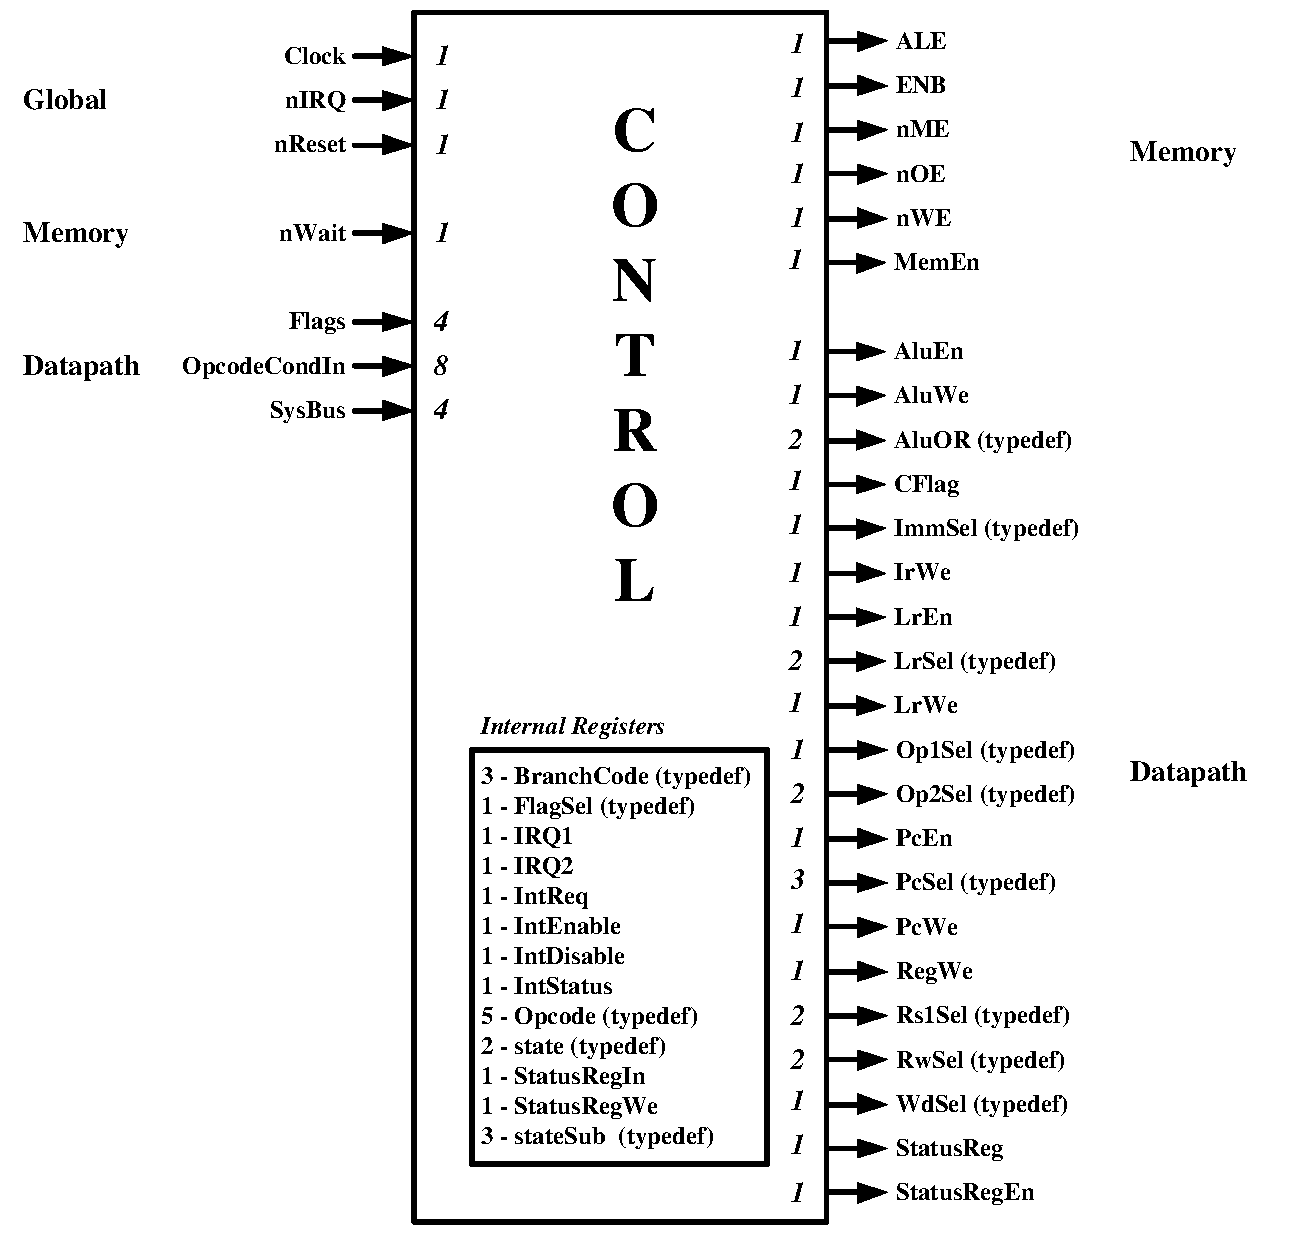
\includegraphics[width = 0.8\textwidth]{ControlPinout.pdf}
		\caption{Inputs, outputs and internal registers of the control block.}% \todo[inline]{Maybe change to IEEE symbols if we have time, AJR: we still have the eagle d-types but I think it would look a bit messy} }
   \label{fig:ControlBlock}
\end{figure}

Three main states exist to service the fetch, execute and interrupt stages.
Five sub states are used within the main states to further coordinate operation.
The ASM chart in figure~\ref{fig:MainStateASM} describes state changes using the sub state, opcode and interrupt request signal.   
When \textbf{nReset} is asserted the machine will return to the first cycle of the fetch state.


\begin{figure}[ht]
   \centering
    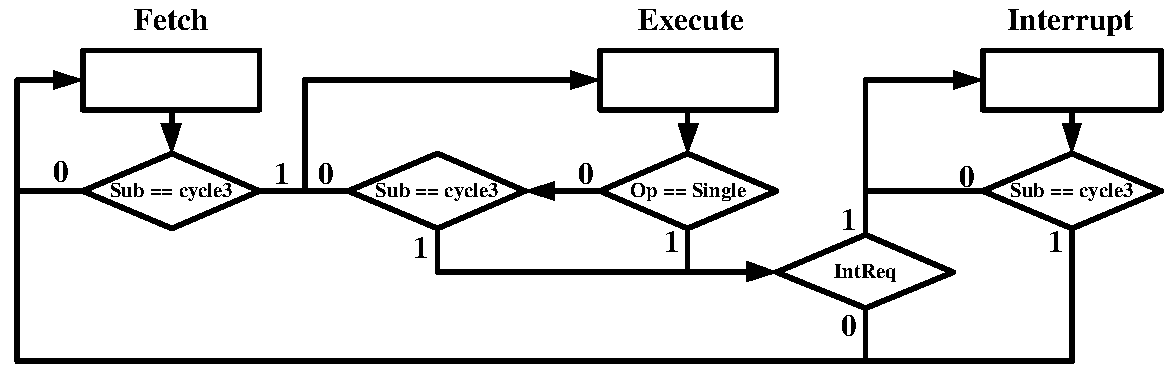
\includegraphics[width = 0.8\textwidth]{MainStateASM.pdf}
		\caption{ASM chart of controller main states.}% \todo[inline]{Maybe change to IEEE symbols if we have time, AJR: we still have the eagle d-types but I think it would look a bit messy} }
   \label{fig:MainStateASM}
\end{figure}








\subsection{Fetch}





\subsection{Execute}




\subsection{Interrupt}


Implementation of interrupts (flags, enable\dots)




\subsection{Synthesis and Layout}

Synthesis and layout - I/O config, magic vs Ledit maybe?
